\section{Q5Cost examples}

Various programs have been implemented using Q5Cost: \texttt{q5dump},
\texttt{cas2hdf}, \texttt{hdf2cost} and, of course, the testsuite presented
in the previous section.

\texttt{q5dump} is a program designed and implemented by Antonio Monari.
It allows access to the information inside a Q5Cost file in a clean and
explicit way. It resembles the \texttt{h5dump} utility from the HDF5
library, but \texttt{q5dump} presents information in chemical speech,
rather than low-level HDF5 concepts like groups and datasets.

A typical output of the program is reported

{\footnotesize
\begin{verbatim}
 ************************************
 *          Q5Costdump              *
 *                                  *
 *     a tool for analysis of       *
 *           Q5Cost files           *
 *                                  *
 ************************************
 
 Creation time 2005/03/30  15.28.05
 
 SYSTEM ATTRIBUTES
 Title: LiHs33                                                          
 Order of the symmetry group  4
 Nuclear Repulsion (Core Energy)  0.995024875621900007
 
 Groups present  2
 ao 1
 tag-default
 mo 1
 tag-default
 ------------------------------------------------------
 
 Properties of AO group <default>
 
 Number of Orbitals 33
 Orbital in Symm. Classes   17   7   7   2
 AO is empty
 ------------------------------------------------------
 
 Properties of MO group <default>
  AO REF: <default>
 
 Number of Orbitals 33
 Orbital in Symm. Classes   17   7   7   2
 
 dipolex is present
 dipolez is present
 oneint is present
 twoint is present
 orbitals is empty
 
 ------------------------------------------------------

\end{verbatim}
}
which can be compared against the output produced by \texttt{h5ls}
{\footnotesize
\begin{verbatim} 
/ao                      Group
/ao/tag-default          Group
/mo                      Group
/mo/tag-default          Group
/mo/tag-default/Property-dipolex Group
/mo/tag-default/Property-dipolex/CompactMatrix-data Group
/mo/tag-default/Property-dipolex/CompactMatrix-data/index Dataset {2, 171/Inf}
/mo/tag-default/Property-dipolex/CompactMatrix-data/value Dataset {171/Inf}
/mo/tag-default/Property-dipolez Group
/mo/tag-default/Property-dipolez/CompactMatrix-data Group
/mo/tag-default/Property-dipolez/CompactMatrix-data/index Dataset {2, 181/Inf}
/mo/tag-default/Property-dipolez/CompactMatrix-data/value Dataset {181/Inf}
/mo/tag-default/Property-oneint Group
/mo/tag-default/Property-oneint/CompactMatrix-data Group
/mo/tag-default/Property-oneint/CompactMatrix-data/index Dataset {2, 182/Inf}
/mo/tag-default/Property-oneint/CompactMatrix-data/value Dataset {182/Inf}
/mo/tag-default/Property-twoint Group
/mo/tag-default/Property-twoint/CompactMatrix-data Group
/mo/tag-default/Property-twoint/CompactMatrix-data/index Dataset {4, 39790/Inf}
/mo/tag-default/Property-twoint/CompactMatrix-data/value Dataset {39790/Inf}
/mo/tag-default/orbitals Dataset {0/Inf, 0/Inf}
\end{verbatim}
}

\texttt{cas2hdf} and \texttt{hdf2cost} are converter utilities, designed to
stress a first deployment of the library in a production environment.  In
Fig. \ref{fig:q5cost-final}, a representation of the final intended
procedure is depicted.
\begin{center}
\begin{figure}[ht]
\begin{center}
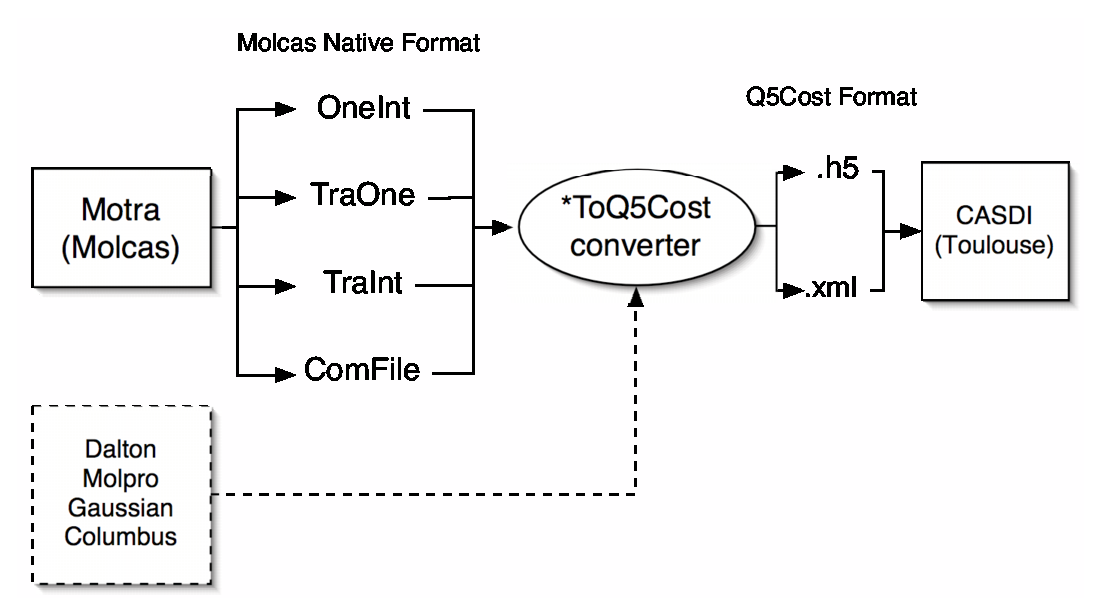
\includegraphics[width=10cm,keepaspectratio]{04_grid/images/q5cost-final-gimped.eps}
\end{center}
\caption{\footnotesize One of the possible final code layouts, involving
direct changes in the code. An integral producer, such as \texttt{MOLCAS}, provides
proprietary files. These files are fed to a converter, which creates the new
Q5Cost format. The program \texttt{CASDI} from Toulouse directly reads these
files. This infrastructure at the moment is not possible, because the
current \texttt{CASDI} implementation reads the old COST format.}
\label{fig:q5cost-final}
\end{figure}
\end{center}

Output integrals are produced by a commercial package, \molcas in the
example, but converters could be developed for other programs, like
\texttt{DALTON}, \texttt{COLUMBUS} and so on. These integrals are fed into a converter to
produce the Q5Cost file format, made of the HDF5 file and an XML (QCML) file
providing additional information. The Q5Cost format will be read by
CASDI, a program from the Toulouse chain of programs. This
approach assumes that \texttt{CASDI} is directly interfaced with the Q5Cost format. 

A more conservative way to handle this interface is represented in Fig.
\ref{fig:q5cost-intermediate}.
\begin{center}
\begin{figure}[ht]
\begin{center}
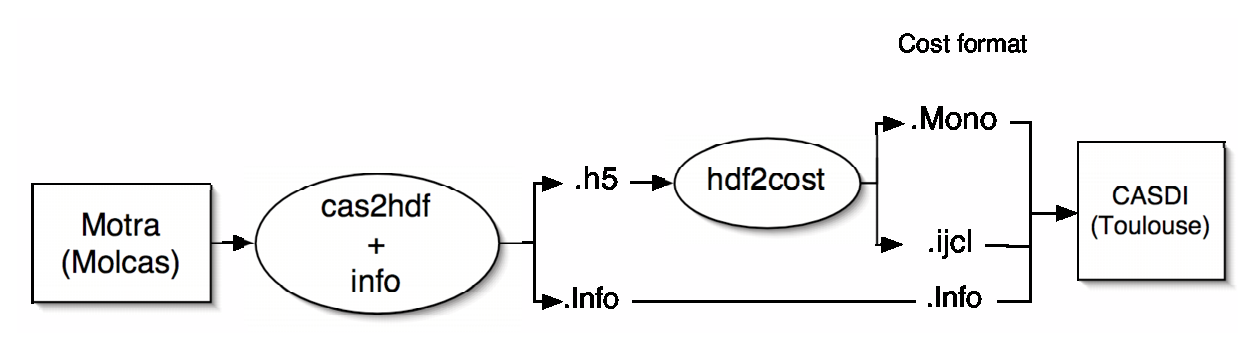
\includegraphics[width=10cm,keepaspectratio]{04_grid/images/q5cost-intermediate-gimped.eps}
\end{center}
\caption{\footnotesize A conservative solution. The \texttt{cas2hdf}
program produces the Q5Cost file, which is converted to the old COST format with
\texttt{hdf2cost}. The \texttt{.Info} file is used as a temporary
replacement of the XML file, and is provided by the \texttt{info}
program, directly interfaced with the \molcas suite. This solution does not
need changes in the CASDI code, and is therefore preferred in the initial
deployment. }
\label{fig:q5cost-intermediate}
\end{figure}
\end{center}

The \texttt{cas2hdf} program directly accesses the \molcas files, producing the
Q5Cost file. The \texttt{.Info} file is used as a temporary replacement of
the XML file, and it is provided by the \texttt{info} program.
The resulting Q5Cost file is read by \texttt{hdf2cost} and converted to the
old COST format, which can be directly read by CASDI.  This solution does
not need changes in the \texttt{CASDI} code, and is therefore preferred in the
initial deployment.

The deployment of these tools made possible to obtain a successful
interface between \molcas and \texttt{CASDI}. Some successful experiment has been also
performed with \texttt{DALTON}.

An experiment of direct integration has been performed with the
\texttt{Full-CI}\cite{cpl-252-437-1996,ijqc-48-287-2004} program developed
in the Professor Bendazzoli research group at Bologna University. The
\texttt{Full-CI} code is now able to read Q5Cost files, and can be
interfaced with both \molcas and \texttt{DALTON}.

